Dieses Kapitel beschreibt der Aufbau der Pixhawk App. Dieses Programm kann völlig losgelöst vom Simulink programmiert werden.


\subsubsection{Statemachine}
Für diese App wurden mehrere Statemachines eingesetzt. Eine übernimmt die komplette Businesslogik für den Ablauf des Programms. Eine zweite Statemachine sorgt dafür, dass die serielle Datenkommunikation korrekt interpretiert wird.


\paragraph{Businesslogik}\mbox{}\\
Die App besitzt zwei Threads. Der Erste ist nur für die Kommunikation und Interpretation der nsh Kommandos verantwortlich. Dieser Thread läuft nur ein paar Zyklen lang und steuert den zweiten Task. Die Steuerkommandos sind start, stop, status, help.\\

\noindent Der zweite Thread übernimmt die gesammte Businesslogik, welche in Abbildung \ref{fig:Statemachine Businesslogik} aufgezeigt wird. In dieser Logik werden jeweils Daten zwischen Interfaces ausgetauscht.\\

\begin{figure}[ht]
  \begin{center}
  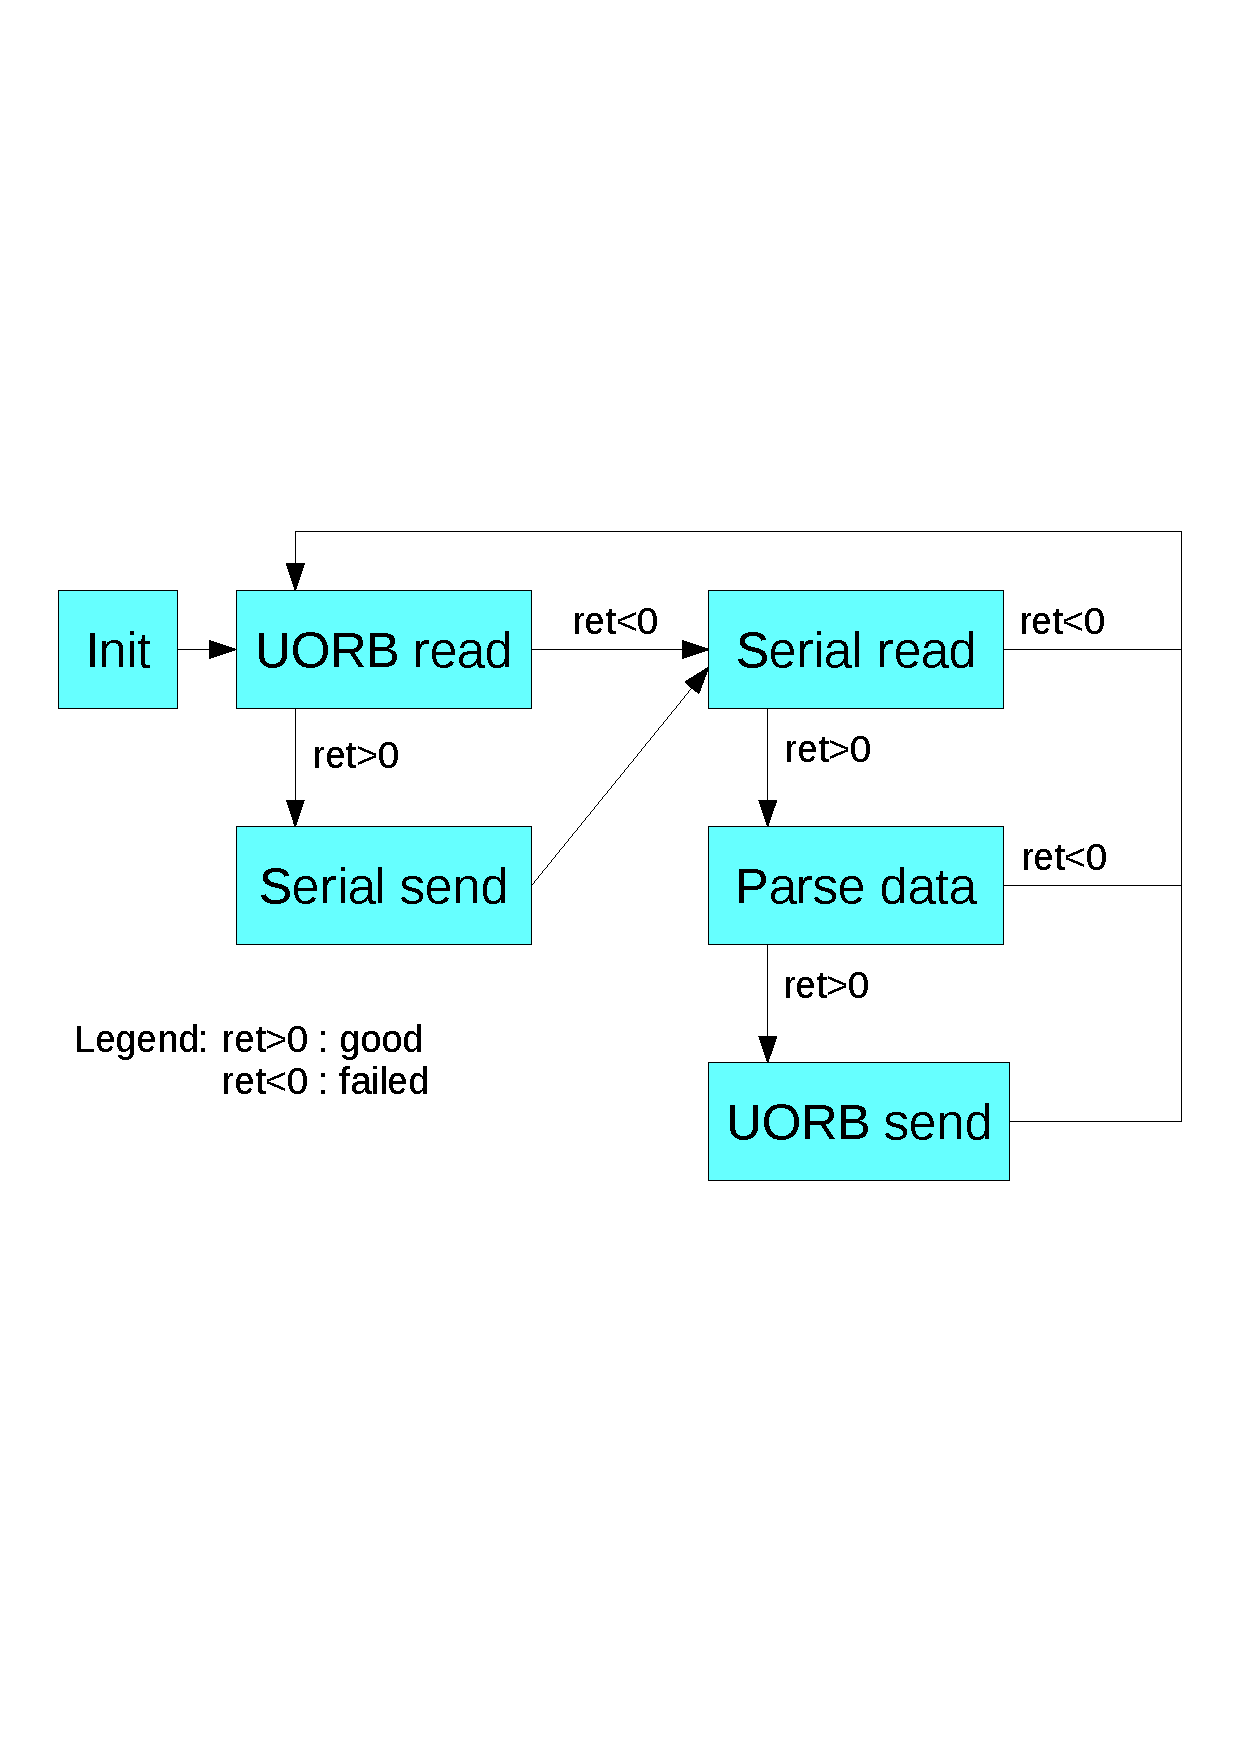
\includegraphics[scale=0.5, trim={1cm 9.5cm 0cm 9cm},clip]{pic/50_app/statemachine_thread.pdf}
  \caption{Statemachine Businesslogik}
  \label{fig:Statemachine Businesslogik}
  \end{center}
\end{figure}

\noindent Nach der Initialisierung werden zwei 2 Hauptaufgaben ausgeführt. Zum einen die uORB Pakete auf die UART übertragen, zum anderen die UART Pakete in die uORB weiterleiten. Dieses Vorgehen ist in obiger Abbildung detailliert erklärt. Die Zustandsfunktionen haben jeweils einen return Wert (ret). Anhand dieses Wertes wird jeweils das weitere Vorgehen bestummen.

\clearpage
\paragraph{Parser}\mbox{}\\

\noindent Die Daten werden jeweils als Paket übertragen. Diese Struktur ist in Abbildung \ref{fig:packet1} aufgezeigt. Eine Erweiterung wäre die ID der Payload zu übermitteln. Dadurch wüsste man, um welches uORB Topic es sich handelt.

\begin{figure}[ht]
	\begin{center}
		\begin{subfigure}{0.49\textwidth}
%			\begin{center}
		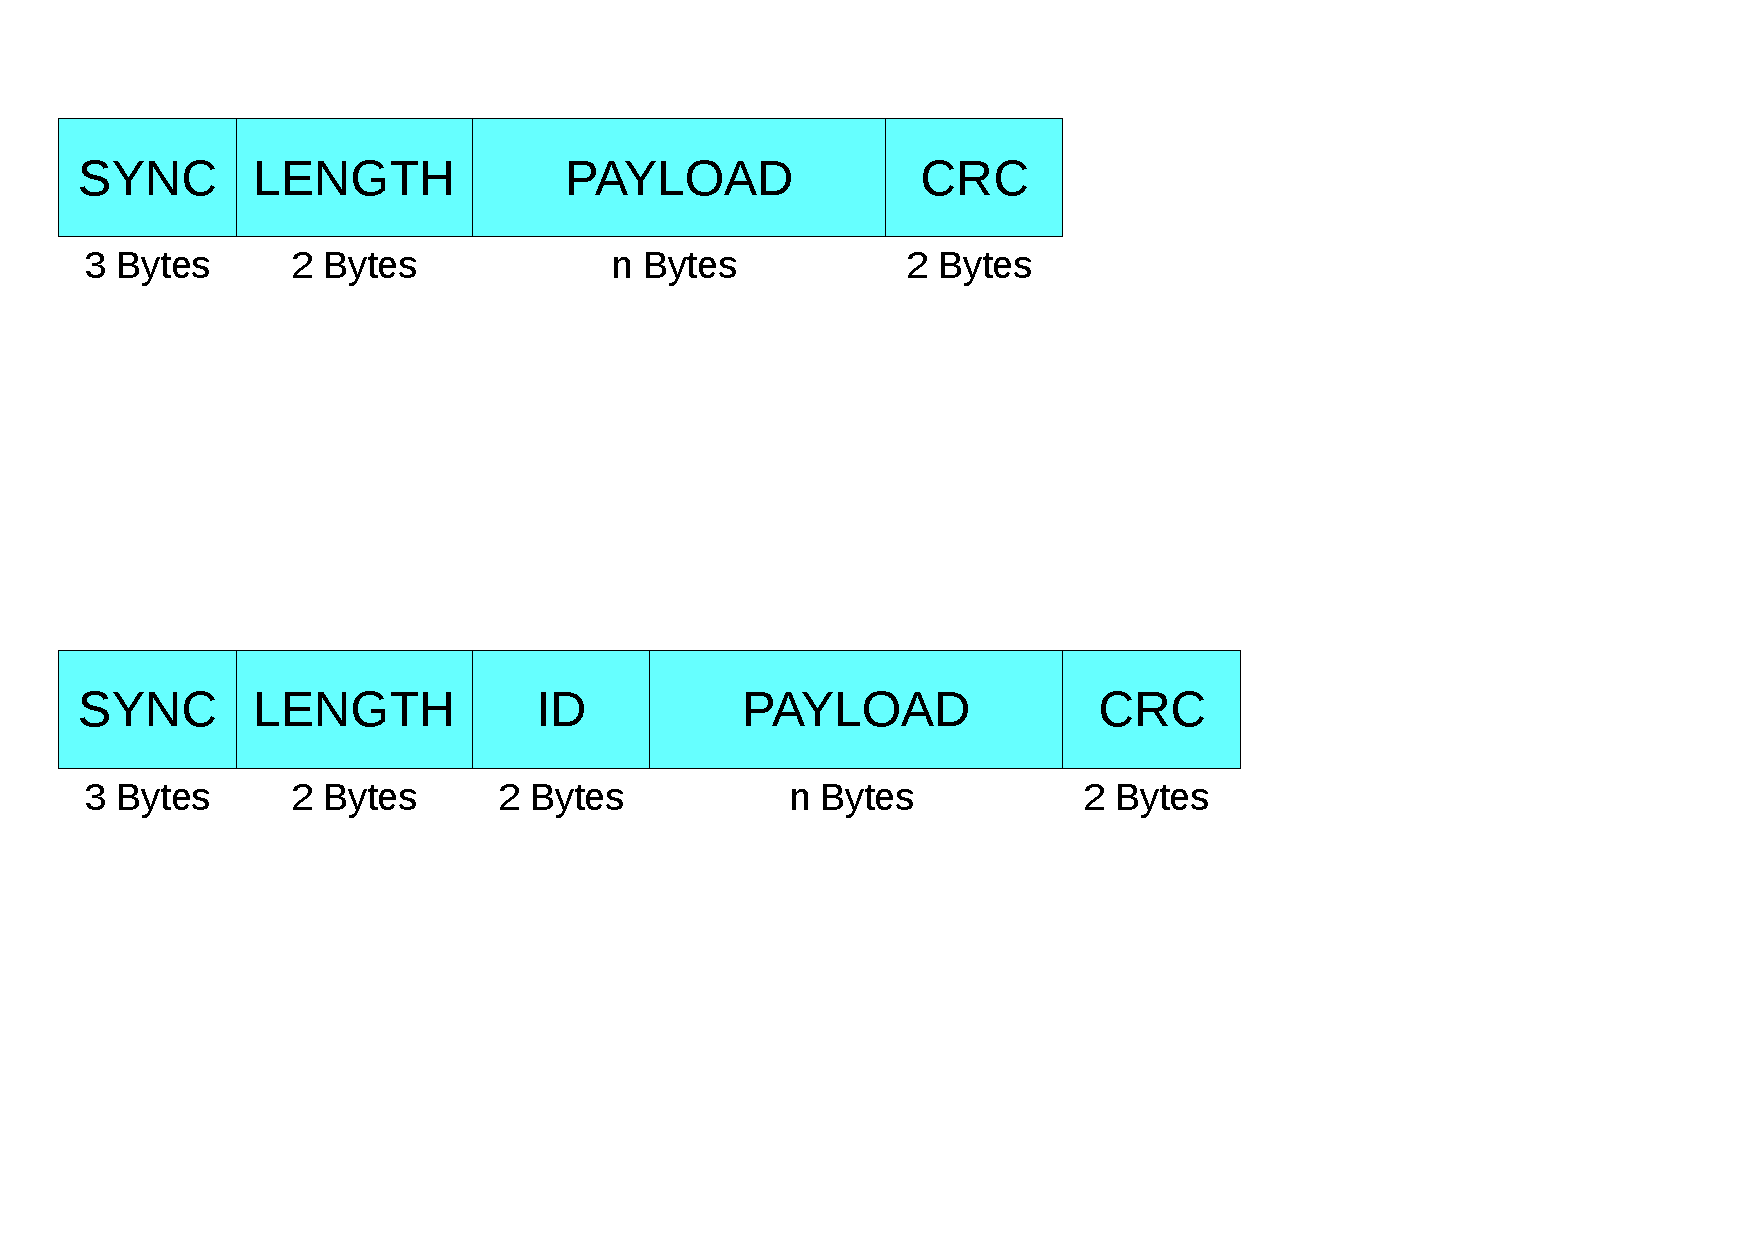
\includegraphics[scale=0.5, trim={0.5cm 16cm 11cm 2cm},clip]{pic/50_app/packet.pdf}
  \caption{Packet Struktur ohne ID}
  \label{fig:packet1}
%		\end{center}
		\end{subfigure}
		
		\begin{subfigure}{0.49\textwidth}
%		\begin{center}
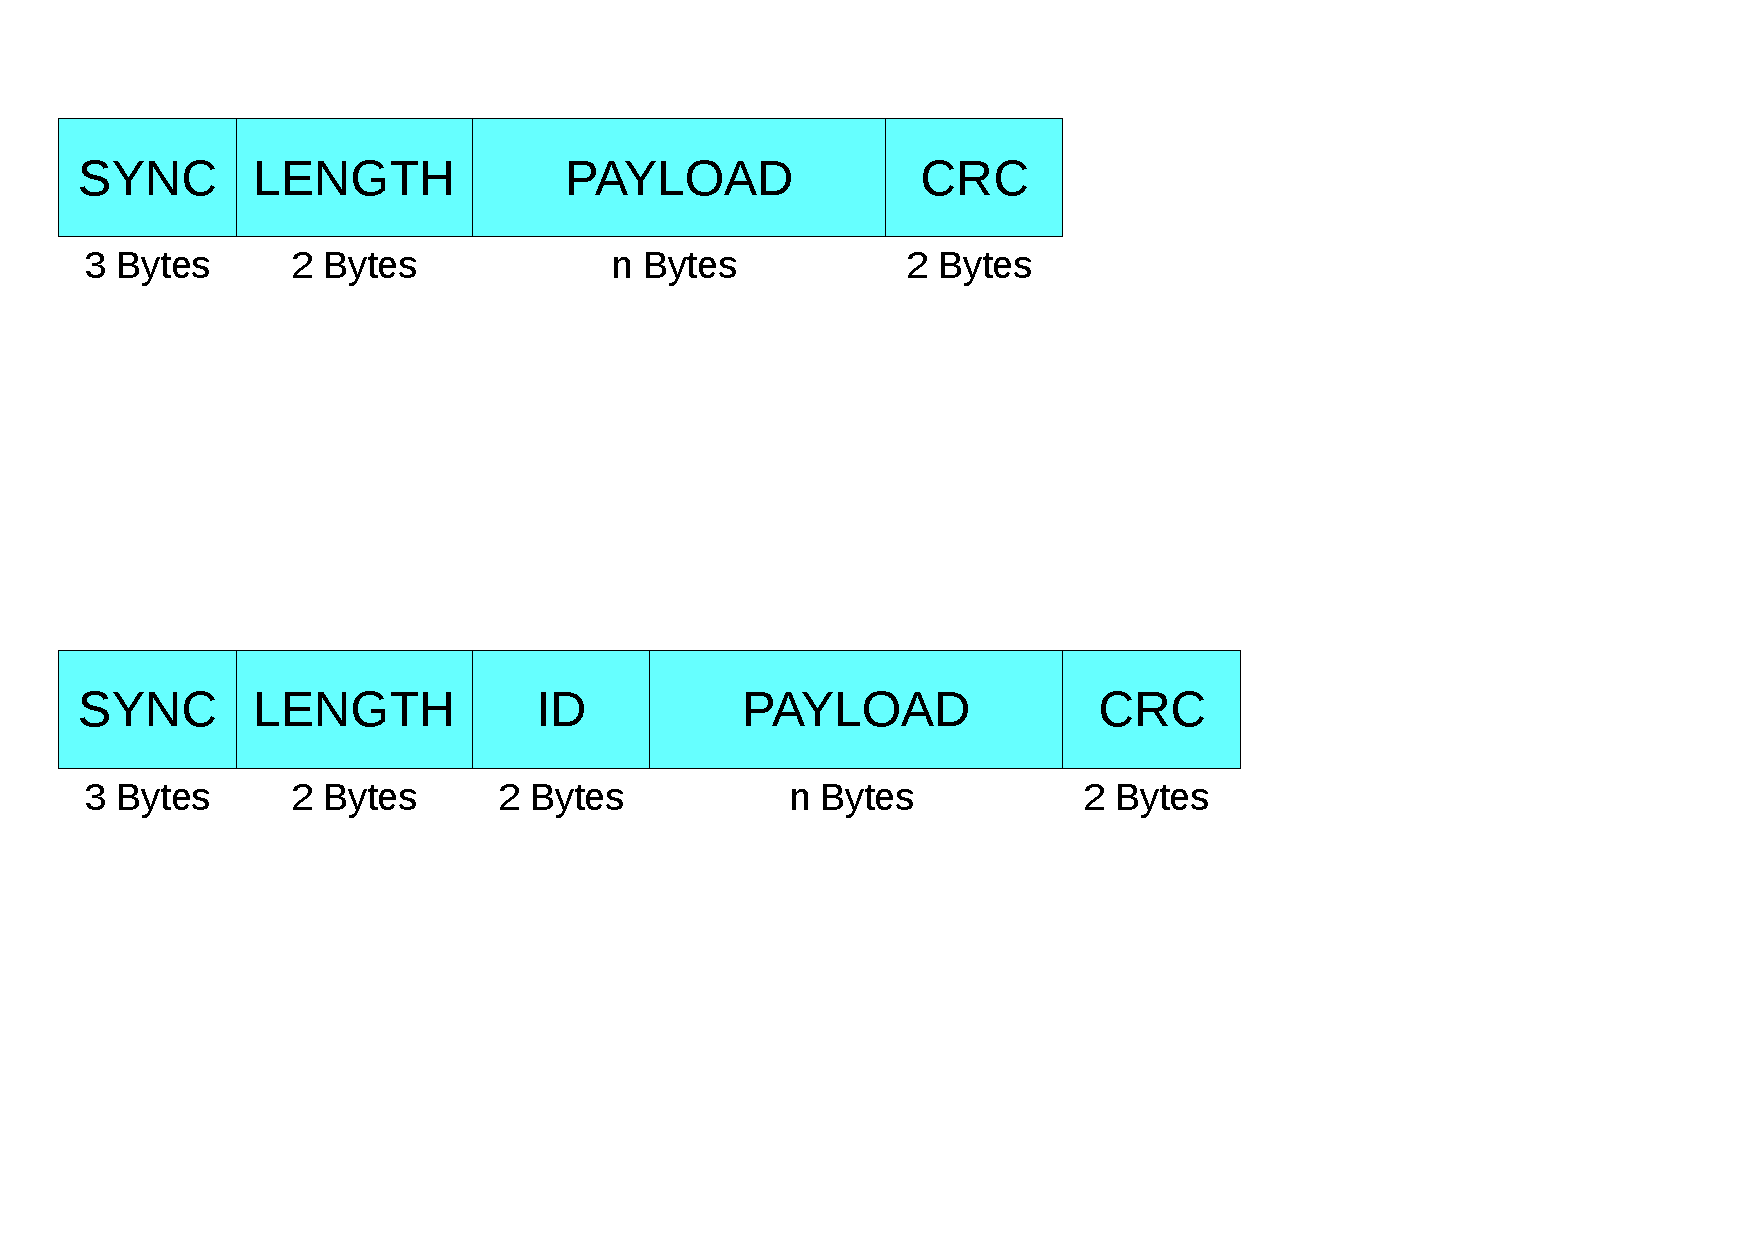
\includegraphics[scale=0.5, trim={0.5cm 7cm 1cm 10.5cm},clip]{pic/50_app/packet.pdf}
  \caption{Packet Struktur mit ID}
  \label{fig:packet2}
%		\end{center}
		\end{subfigure}
		
		\caption{Packetstruktur}
		\label{fig:Packet Struktur}
	\end{center}
\end{figure}


\noindent Die genaue Paketstruktur ist in folgender Tabelle aufgezeigt. Es handelt sich um das 'little Endian' Format. 
\begin{table}[ht]
\begin{center}
  \begin{tabular}{| c | l | c |}
    \hline
    Name & Inhalt & Länge (Byte) \\
    \hline
    SYNC  & Synchronisationszeichen  & 3 \\
          & ASCII: \#:\_                          &  \\
    \hline
    LENGTH & Länge & 2 \\
           & Bytelänge der Payload &  \\
    \hline
    ID & Identifikation: & 2 \\
       & Bit Array, bei welchem jedes Bit einem definierten uORB Topic entspricht.&  \\
    \hline
    PAYLOAD & Nutzdaten & n \\
            & Daten im roh Format & \\
    \hline
    CRC & Checksumme & 2 \\
        & CRC16 über die SYNC, LENGTH, (ID) und PAYLOD Daten & \\
    \hline
  \end{tabular}
  
  \caption{Paketstruktur Beschreibung}
  \label{tab:Paketstruktur Beschreibung}
  
\end{center}
\end{table}

\noindent Durch die ID kann festgelegt werden, welche uORB Topics in der PAYLOAD vorhanden sind. Damit alle Permutation möglich sind, ist jedem ID-Bit ein uORB Topic zugewiesen.

\begin{table}[ht]
\begin{center}
  \begin{tabular}{| l | l |}  
    \hline
    Bits [MSB ... LSB] & uORB Topic Name \\ \hline
    1xxx'xxxx xxxx'xxxx & Heartbeat\\ \hline
    x1xx'xxxx xxxx'xxxx & Sensor combined \\ \hline
    xxxx'xxxx 1xxx'xxxx & Actuator armed \\ \hline
    xxxx'xxxx x1xx'xxxx & Actuator controls \\ \hline
  \end{tabular}  
  \caption{Paket ID}
  \label{tab:Paket ID}  
\end{center}
\end{table}


\clearpage
\noindent Bei den empfangenen Daten muss zuerst der Beginn festgelegt werden. Für dies wird eine Parser (Abbildung \ref{fig:Statemachine Parser} verwendet.


\begin{figure}[ht]
  \begin{center}
  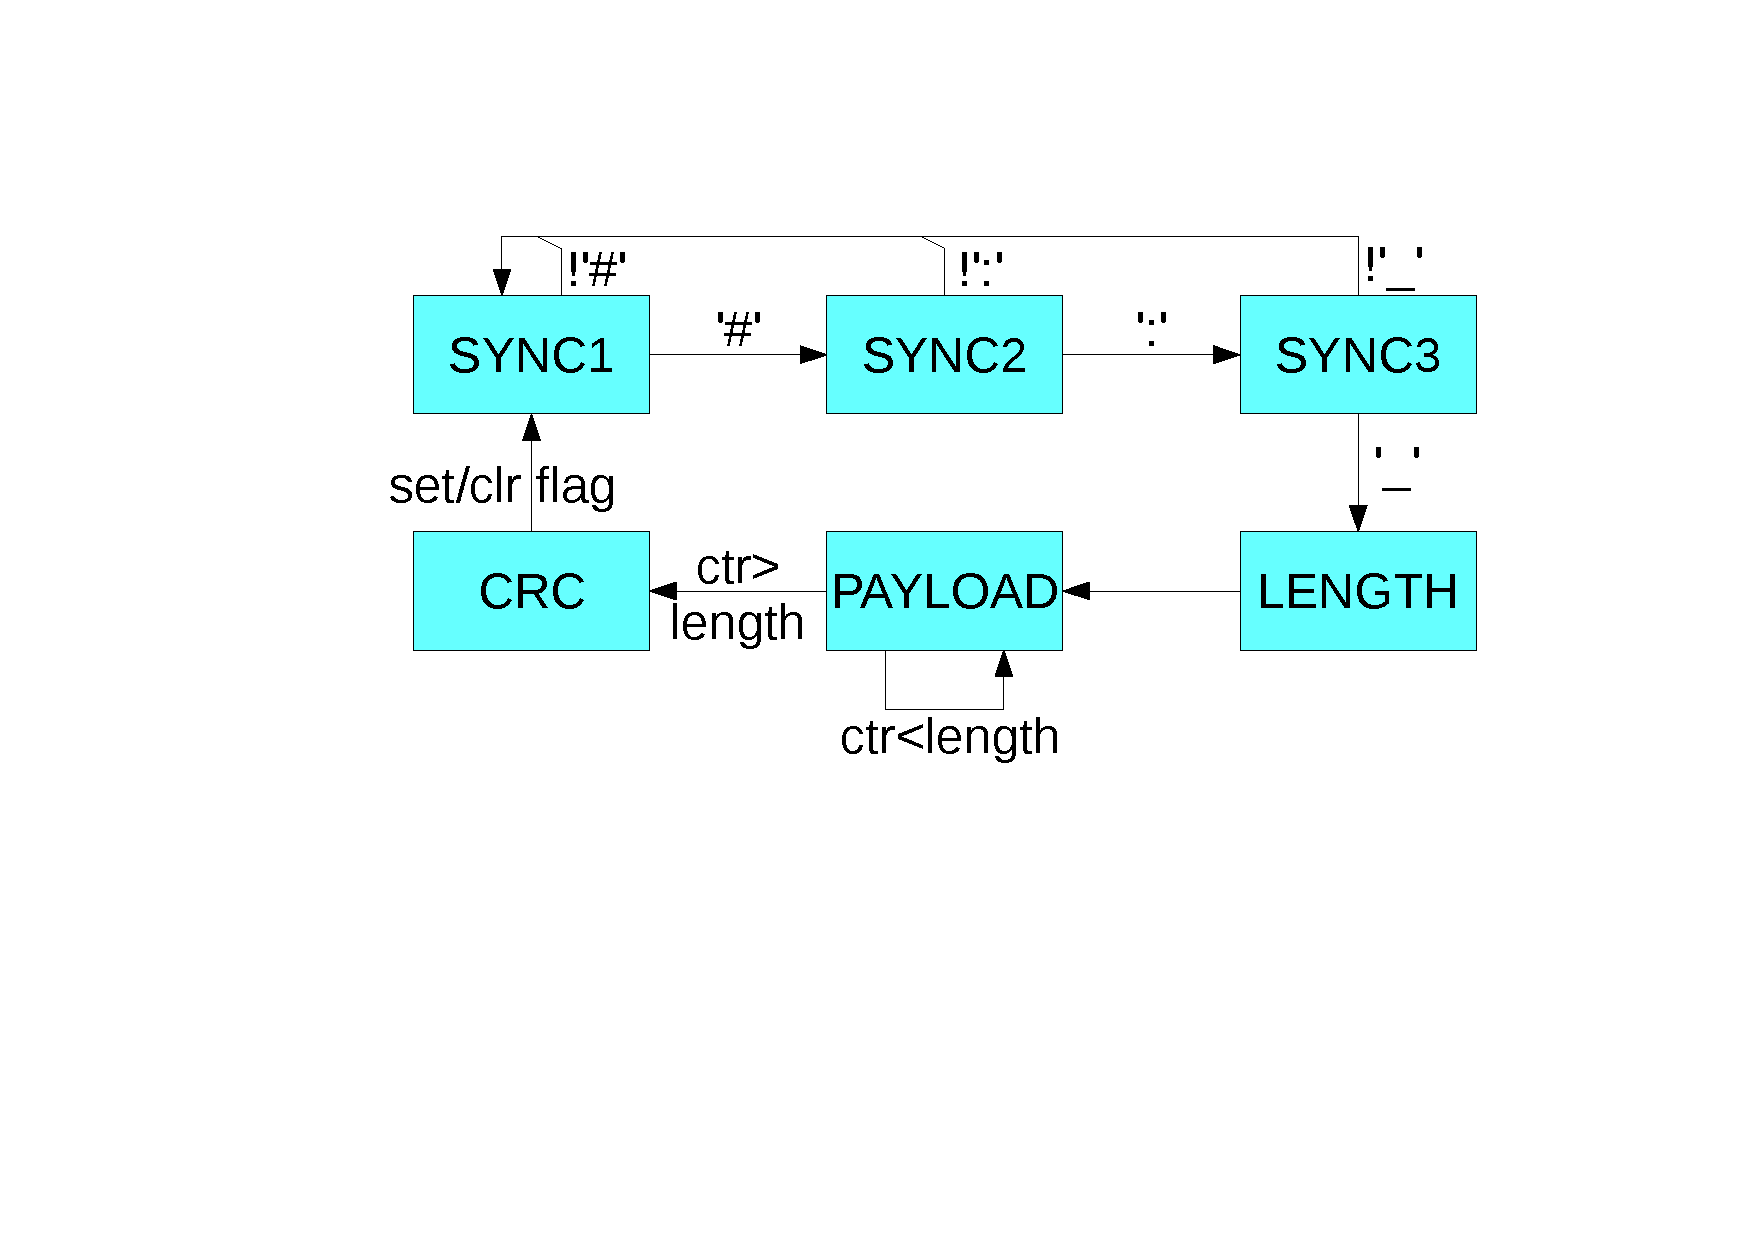
\includegraphics[scale=0.5, trim={6cm 8cm 4cm 4cm},clip]{pic/50_app/statemachine_parser.pdf}
  \caption{Statemachine Parser}
  \label{fig:Statemachine Parser}
  \end{center}
\end{figure}

\noindent Die Synchronisationsreihenfolge \#:\_ wurde desshalb gewählt, da diese eine zufällige Reihenfolge an Bits enthält. Weiter ist die Chance, dass dieses Bit-Reihenfolge erscheint $P = \frac{1}{2^{3\cdot8 Bits}}\approx\frac{1}{16\cdot 10^6} \approx 6 \cdot 10^{-8}$. Weiter sollte diese Reihenfolge im ASCII Format leicht ersichtlich sein, um das Debuggen zu vereinfacht. ASCII Steuerzeichen wurden bewusst nicht verwendet, da diese ja nach Betriebssystem, sowie Programm anders interpretiert werden können. \\
Am Ende des Pakets wird eine CRC16 mit dem Polynom $0x8005 = x^{16} + x^{15} + x^2 + 1$ angehängt. Durch Verwendung von nur einer Checksumme kann der Fehler im Paket nicht lokalisiert und korrigiert werden. Für die HiL Simulation steht die Geschwindigkeit jedoch im Vordergrund. Falls die Checksumme nicht übereinstimmt, wird das gesamte Paket verworfen.

\clearpage
